\documentclass{llncs}
\usepackage{graphicx}
\usepackage{color}
\usepackage{hyperref}
\usepackage[utf8]{inputenc}
\hypersetup{
    colorlinks=true,
    linkcolor=blue,
    filecolor=magenta,      
    urlcolor=cyan,
}
%%%%%%%%%%%%%%%%%%%%%%%%%%%%%%%%%%%%%%%%%%%%%%%%%%%%%%%%%%%%%%%%%%%%%%%%%%
\usepackage{todonotes} % use this to see the comments
%\usepackage[textsize=tiny]{todonotes} % use this to see SMALL : ) comments
%\usepackage[disable]{todonotes} % use this to hide all comments
%%%%%%%%%%%%%%%%%%%%%%%%%%%%%%%%%%%%%%%%%%%%%%%%%%%%%%%%%%%%%%%%%%%%%%%%%%


\newcommand{\todoinline}[1]{
    \todo[inline]{#1}
}
\newcommand{\todoiteminline}[3]{
    \todoitemtemplate{#1}{#2}{#3}{inline}{red}
}

\newcommand{\todoproofread}[3]{
    \todoitemtemplate{#1}{#2}{Please proof read above section; #3}{inline}{yellow}
}
\definecolor{mygreen}{HTML}{00CC00}
\newcommand{\todoproofreadDone}[3]{
    \todoitemtemplate{#1}{#2}{Please proof reading above section, done; #3}{inline}{mygreen}
}
\newcommand{\todoproofreaddone}[3]{
    \todoproofreadDone{#1}{#2}{#3}
}

\newcommand{\todoitemtemplate}[5]{%
% \index[MYTODO]{#2}
\todo[#4,color=#5,caption=X]{{#1}{ \textbf{{\tiny{for}} #2}:}{#3}}%
}

\newcommand{\todoiteminlinedone}[3]{
    \todoiteminlineDone{#1}{#2}{#3}
}
\newcommand{\todoiteminlineDone}[3]{
    \todoitemtemplate{{\commentsDoneFont{#1}}}{{\commentsDoneFont{#2}}}{{\commentsDoneFont{#3}}}{inline}{green}
}

\newcommand{\todoitem}[3]{
    \todoitemtemplate{#1}{#2}{#3}{}{red}
}
\newcommand{\todoitemdone}[3]{
    \todoitemDone{#1}{#2}{#3}
}
\newcommand{\todoitemDone}[3]{{\commentsDoneFont\todoitemtemplate{{\commentsDoneFont{#1}}}{{\commentsDoneFont{#2}}}{{\commentsDoneFont{#3}}}{}{green}}}


\begin{document}



%\title{All about Indexing for Question Answering systems: A deep dive into Information retrieval}
%\title{Graph vs RDF stores: An Empirical Evaluation of NoSQL RDF Data Management Solutions}
%\title{An Empirical Evaluation of NoSQL RDF Data Management Solutions}
%\title{Benchmarking RDF Data Management Solutions}
\title{LITMUS: An Open Extensible Platform for Benchmarking RDF Data Management Solutions}


\author{Harsh Thakkar\inst{1}, Mohnish Dubey\inst{1}, Gezim Sejdiu\inst{1}, Axel-Cyrille Ngonga Ngomo\inst{2}, Jens Lehmann\inst{1,3}, S\"{o}ren Auer\inst{1,3}\dots}
\institute{
	Institute for Computer Science III, University of Bonn;\\ 
	\email{\{thakkar,dubey,sejdiu,jens.lehmann,auer\}@cs.uni-bonn.de}
	\and 
	University of Leipzig;\\
	\email{ngonga@informatik.uni-leipzig.de}
	\and 
	Fraunhofer IAIS;
	\email{jens.lehmann@iais.fraunhofer.de}
\vspace{-8pt}
	}
\maketitle

\begin{abstract}

Advancements in the field of Linked data have led to an enormous outburst of structured data. To keep up with the pace of efficient consumption and management of the data at this rate, many Data Management Solutions (DMS) have been developed for specific task and applications. \dots 
\todoiteminline{Harsh}{co-authors}{Please contribute in the abstract writing}

\end{abstract}

\section{Introduction}\label{sec:Introduction}
     
    \todoiteminline{Harsh}{co-authors}{This might need re-phrasing, feel free to do so}
    
    The current era stands as a witness to the enormous explosion of structured data on the Web referred to as Linked Data\footnote{http://lod-cloud.net/}. With such a rapid growth in the amount of data, managing this data has also become a challenging issue. Modern day organizations have become increasingly interested in searching for data management solutions, suited best for their needs, based on Linked Data. Choosing the best data management solution has become a problem analogous to searching for a needle in a gigantic haystack. With limited domain expertise, apriori information and non-stop expansion of data the need for a standardised framework to benchmark and analyse the existing diverse data management solutions has become more critical. 
    
    \todoinline{one more paragraph to be added here about some current activity, etc on benchmarking platforms if suitable}
    Despite growing interest and use in both research communities and industries, current DMS benchmarks do not offer a common suite for creating benchmarks and no single baseline on how to compare one against the other. Moreover, re-producing or replicating benchmarks, created by others, is a non-trivial problem owing to reasons such as, non-standardised setup configurations, lack of publicly available resources (such as scripts, packages, etc) and lack of transparent evaluation policies. 
    %due to a variety of reasons including (i) unclear setup configuration, (ii) non-standard . as the unit of verification of the results for a whole systems. 
    %In order to fill the gaps (i) to help end user to choose the right system by showing the ranked results of the system's behaviors for the different parameter selection permutation, and (ii) the involvement of industry community to improve their systems by modeling a different challenges and pick a right pipeline for their needs.
    
    There have been many research efforts in the direction of benchmarking a range of DMS, including some which have also considered evaluating cross domain DMS {cite graphium, pandora}, but only to a limited scope. \todo[color=green]{Harsh: working on this, Need to add more information here..}
    
    
    In this paper we present LITMUS, an open extensible solution towards benchmarking a wide variety of NoSQL data management solutions (DMS). LITMUS is focused to to support organizations/institutions which aspire to use Linked Data management technologies in a wide spectrum of applications and magnitudes. 
    LITMUS will provide realistic performance evaluation platform covering a plethora of heterogeneous technologies (see Section~\ref{litmus_framework}) for storage and querying benchmarking. The objectives of LITMUS are to:
     \begin{itemize}
        \item provide a common transparent platform to benchmark, compare and analyse cross domain Data Management Solutions (DMS) wrt to a wide variety of data and queries;       
        \item serve as an open extensible framework for allowing easy replication, integration and evaluation of existing benchmarks for an existing plethora of tools;
        \item explore and study a wide range of storage and indexing techniques used by existing DMS and their correlation with a wide spectrum of performance indicators
      \end{itemize}
    
        This paper is organised as follows: We briefly present a survey on the existing benchmarking efforts involving relational databases, graph/RDF data management, Linked Data integration approaches and instance matching domains and motivation are presented in Section~\ref{relwork}. Then in Section~\ref{Objectives} we go throw light on the focus of LITMUS, the challenges to be addressed and the target communities which can benefit from LITMUS. We present the LITMUS framework and describe the components in brief in Section~\ref{litmus_framework}.  




%========================================RELATED WORK======================================
\section{Related work}\label{relwork}

    Benchmarking is widely used for evaluating data stores, and benchmarks exist for a variety of levels of abstraction, from the data graphs, to the triple stores, even to complete enterprise systems.
    By understanding and describing the current state of the art in benchmarking; in particular, benchmarks for (a) relational databases, (b) graph databases, (c) key-value stores, (d) wide column stores.
    
    By doing this, we identify shortcomings and limitations of existing systems in order to employ LITMUS by extending these benchmarks to deal with the challenges forces by new systems.
    Thus, in addition to surveying existing work, we intend to focus mainly on the purpose and scope of the benchmarks.
    
    The most popular model of relational databases have standard benchmark suites such as TPC~\cite{Nambiar2011} benchmark dealing with transaction processing, querying performance, data maintenance and other operations for a relational database.
    
    The TPC~\cite{Nambiar2011} benchmark suit deals with transaction processing, querying performance, data maintenance and other operations for a relational database.
    However, its general abstraction is not suitable for other data models, as they have been specifically made for relational databases.
    
    For benchmarking functions of graph databases, there are some existing techniques on their early stages (such as HPC Scalable Graph Analysis Benchmark~\cite{Dominguez-Sal:2010:SGD:1927585.1927590}, Graph 500~\cite{murphy2010introducing}, XGDBench~\cite{conf/cloudcom/DayarathnaS12}) dealing with graph suitability and graph analysis and they fail on defining standards for graph modeling and query languages.
    
    Existing RDF benchmarks have several limitations, mainly because they do not provide enough metadata for representing datasets, and support only some type of queries.
    In this context there is some work done on data integration benchmarks, mainly on entity annotation where GERBIL~\cite{Usbeck:2015:GGE:2736277.2741626} offers an easy-to-use platform for the agile comparison of annotators using multiple datasets and uniform measuring approaches.
    
    Recently, the ongoing work at LDBC council \cite{DBLP:journals/sigmod/AnglesBLF0ENMKT14} try to combine benchmarks for graph and RDF data management systems.
    
    However, we felt it was necessary to define a new benchmark for Linked Data Systems. First, most data stores do not have an interface which allow user to execute SPARQL queries against any kind of end data structure representation, or they only support a subset of operations.
    Toward, the complex queries of many existing SPARQL benchmarks were not applicable. Secondly, the use cases of Linked Data are often different than traditional database applications, so that narrow domain benchmarks may not match the intended usage of the system.
    Furthermore, our goal is to develop a benchmarking framework that could be used to explore the performance space of different systems, rather than to measure a single performance number representing a particular application.
    
    Designing an accurate and scalability benchmark, and force its usage to gather accurate results, is non-trivial. 
    
    There is a lack of effort to benchmark and compare Data Management Solutions (DMS) from cross domains. There exist no such open, extensible and reusable framework exists to the best of our knowledge which allows to explore, analyse and play with a wide range of DMSs.
    Our aim is to satisfy these criteria by developing a benchmark to serving systems, portable to different end data structure representation through our extensibility framework, scalable to large scale data sets, and employing any kind of operations on top of it.
    
    
    \todoproofread{Gezim}{all}{and Review too}

    
   % \begin{itemize}
   %     \item survey papers and other formal publications on benchmarking different graph stores, comparison of various triple stores and so on
    %    \href{https://docs.google.com/document/d/1DbtHvE4oaSuusPjeM2nGNBzrRArQt_rlCh3J5g2aIAE/edit?usp=sharing}{Literature review of Related Work}
        
    %    \item Papers on data, queries and other tools used for benchmarking
%    \end{itemize}
    
    
   % {\color{red}{Other benchmarks, Other such frameworks? LDBC council work to be cited Gerbil to be cited BAT-framework to be cited }}

\section{Objectives, Challenges and Outcomes}\label{Objectives}

    \subsection{Focus of the LITMUS framework}
    The LITMUS framework aims at bridging the gaps in adopting, deploying and scaling the consumption of Big Linked Data. LITMUS is being built with a dedication to simplify the use, assessment and analysis of the performances of a wide spectrum of Linked Data management solutions for satisfying the end user's needs.  In particular, the LITMUS project will create: (i) A common ground for carrying out benchmarks for a plethora of cross domain DMS's (ii) Specific benchmarks for the selected DMS's (in the later phases), and  (iii) Reports and scientific studies on the correlation of a wide of factors (query typology, Indexing data structures used~\cite{shekarpour2016question}, etc) affecting the performances of the DMS's. The LITMUS framework will also, during its final phase, be able to serve as a recommendation medium for suggesting particular DMS's for the user specific setting or application based on predefined requirements. 
    
    \subsection{Challenges to be addressed}
    In order to develop such an open extensible benchmarking platform (LITMUS), there are three key challenges which have to be addressed. We describe them in brief as follows:
        \begin{enumerate}
            \item \framebox[1.1\width]{\textbf{C1}}\textbf{ Data conversion}: This challenge demands a generic data conversion mechanism. This will allow the user to convert the input data to a format interpretable by the corresponding DMS (e.g. RDF to CSV (Comma Separated Value), JSON (JavaScript Object Notation),  and SQL (Structured Query Language).
            \item \framebox[1.1\width]{\textbf{C2}} \textbf{Query Conversion:} 
            One of the substantial research gap is the language (query language) barrier. Since all query languages are different in a their structure and expressivity, and the DMS have different query languages, there is a need to develop an intermediate mechanism to convert or express the logic of one query (from one format \textit{say} SPARQL) to the other respective language (\textit{say} CYPHER, SQL, CQL, etc). For instance, path queries (in SPARQL) cannot be expressed in an equivalent manner in SQL. This requires an exhaustive study of the expressivity of query languages and a formal analysis of how they can be mapped to other languages without altering the meaning of the query. This study will provide us with deep insights about the functionality of various query languages, their strengths and limitations.
            also propose a solution approach in the block diagram (as mentioned above).
            \item \framebox[1.1\width]{\textbf{C3}} \textbf{Performance measures/indicators:} 
            The performance of a DMS can be assessed on a wide variety of metrics/features/indicators. It is necessary in order to conduct a correlational analysis of the impact of the diversity in queries and data on storage and indexing efficiency of the DMS. Apart from the traditional performance measures such as precision, recall, index size, storage size, number of triples, query response time, etc there is a need to explore more complex indicators of performance to successfully determine their correlation with the type of data and queries.
        \end{enumerate}
    
    \subsection{Research gaps to be filled by LITMUS}
    The artifacts produced by the research and development activity to be undertaken for the LITMUS project can be grouped into two groups: \textit{(A1)} scientific studies/surveys and \textit{(A2)} software deliverables. 
    
    \framebox[1.1\width]{\textbf{A1}}\textit{ Scientific studies/surveys such as:} 
        \begin{itemize}
            \item Survey of the query language expressivity and features for overcoming the language barrier
            \item A study of a wide range of indexing and storage techniques used for fast and efficient retrieval of structured data
            \item A detailed study of performance features/indicators in the domain of query and data over RDF (structured) data. On top of the existing performance evaluation measures, we will study and analyse a series of other features such as the design of indexes and corresponding data structures on the retrieval performance for structured data. A detailed examination of the correlation between query typology and data storage and retrieval mechanisms.
        \end{itemize}
        
        \framebox[1.1\width]{\textbf{A2}} \textit{Software deliverables (i.e. algorithm(s), tools, etc) including:} 
        \begin{itemize}
            \item A mechanism/range of solutions for converting RDF data to multiple data formats, such as: CSV, JSON, SQL, etc to ensure compatible data input for cross domain DMS's. 
            \item A novel SPARQL to any query language converting algorithm
            \item A wrapper allowing easy integration and deployment of third party DMS's for realistic benchmarking
            \item A universal benchmarking platform: We will develop an open extensible framework for cross domain performance evaluation of query and storage in RDF DMS's. The proposed benchmark will be scalable for large scale evaluations (such as Big Data).
                \todoproofread{Harsh}{all}{and Review too}

    \subsection{Target audience}
        \begin{itemize}
            \item \textbf{Technology Vendors:}
            One of the profiteers from this work will be the Industrial/Commercial fraternity (such as system and data analysts, system developers, system architects) who thrives towards developing advanced DMS for an efficient consumption of Big Linked Data.
            \item \textbf{Technology Consumers:}
            The user's (personnel from the private and commercial organisations, associations, etc ) searching for the best solution for their needs can simply compare a wide range of DMS against a spectrum of desired parameters (types of queries, data, performance indicators) and choose the optimal one for their needs. 
            \item \textbf{Technology Researchers:}
            This includes the researchers who can benefit by absorbing the knowledge and contributing to the rigorous research efforts to for the research community. The target research audience will be the communities, not limited to Semantic Web, Database, Information Retrieval, Big Data researchers, etc.
        \end{itemize}
        \todoproofread{Harsh}{all}{and Review too}


%========================================THE BENCHMARK FRAMEWORK======================================
\section{The Litmus Framework}\label{litmus_framework}
   % \subsection{Objectives}
   %    \todoinline{Needs to formulated well, suggest changes} 
   %   Why are we doing this? - To develop an Open, Extensible and Reusable cross domain platform for:
   %  \begin{itemize}
   %     \item Benchmarking data management solutions across a wide variety of categories
   %    \item Exploring and studying a wide range of storage and indexing techniques and their correlation with different types of queries and data
   %   \item Allowing easy integration and benchmarking of new third party data management solutions to an existing plethora of tools
   %   \end{itemize}
        

    \subsection{Architecture Overview}
        The LITMUS architecture comprises of four major facets or components: Data Facet (F1), Query Facet (F2), System Facet (F3) and the Benchmarking core (F4). Figure \ref{fig:benchmark_arch} illustrates the abstract workflow of the LITMUS framework. We now explain the role of each facet. 
         
        \begin{figure}[h]
            \centering
            %\includegraphics{}
            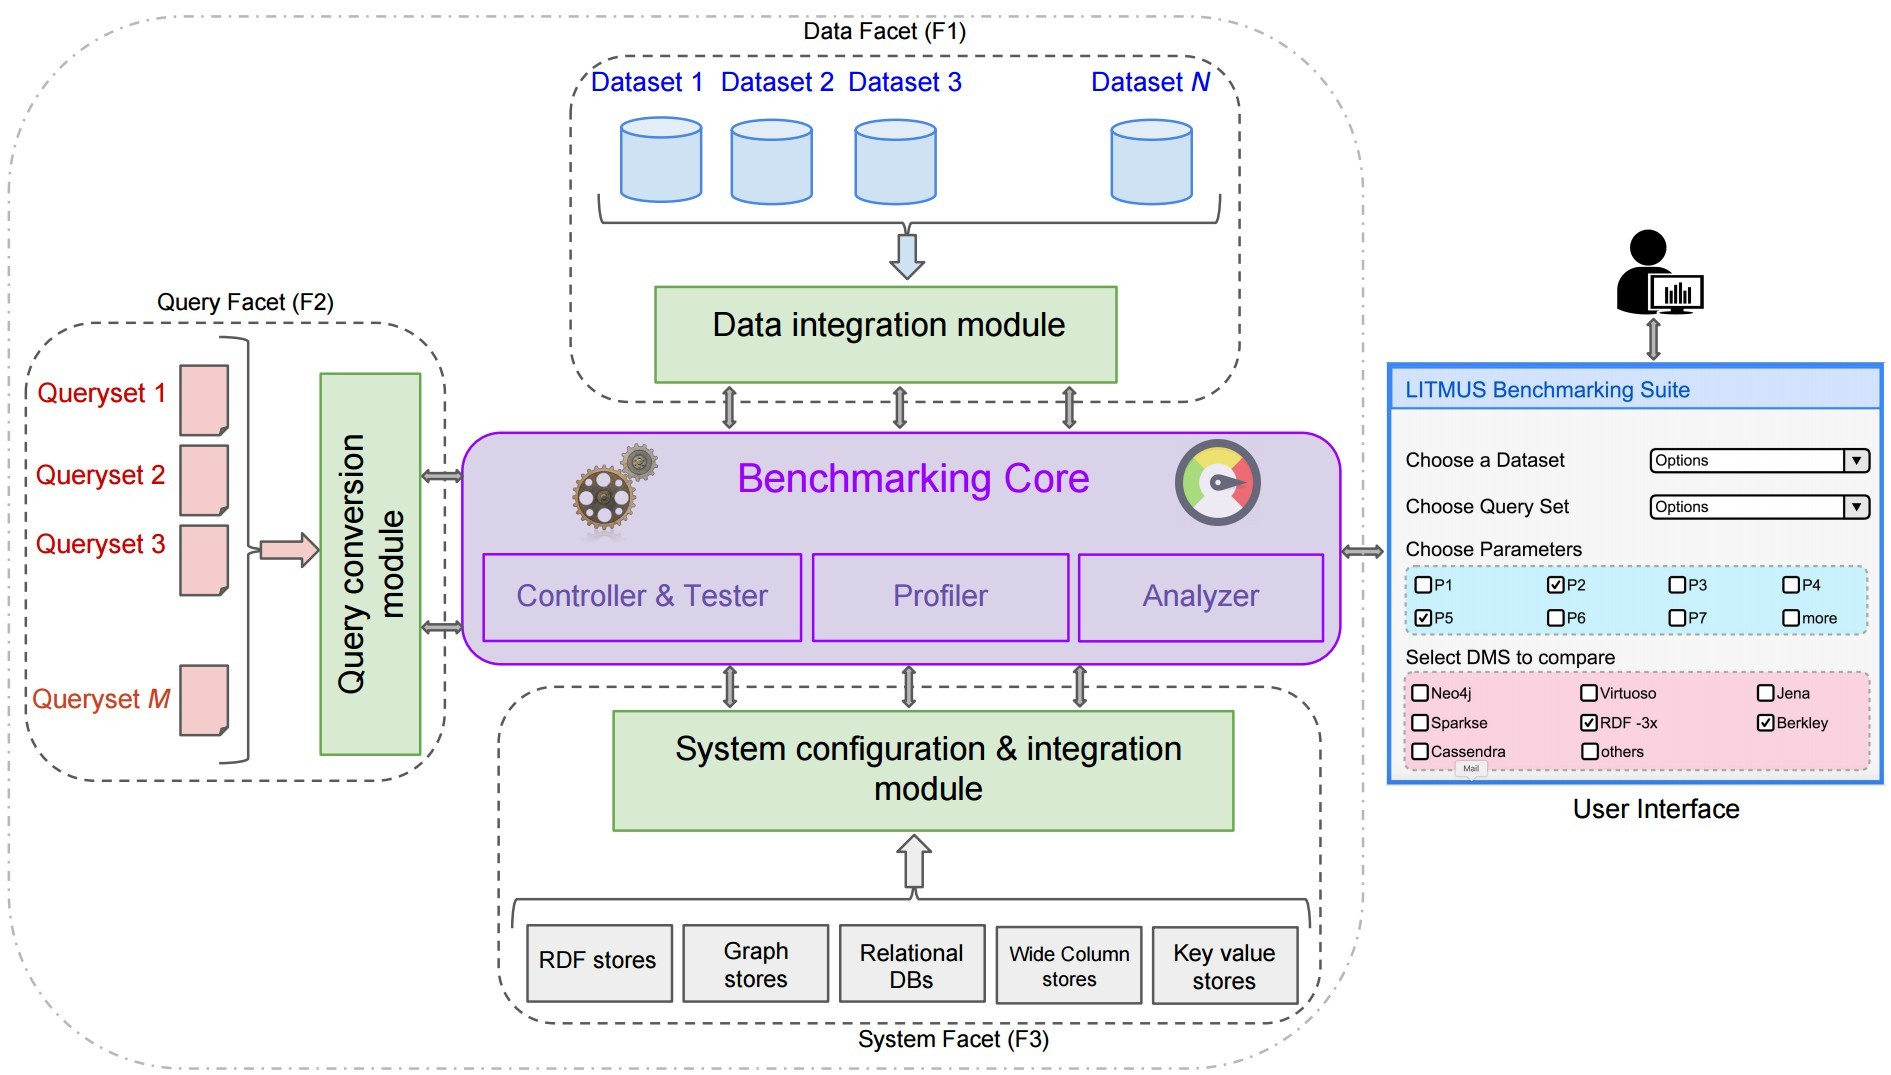
\includegraphics[scale=0.2]{images/benchmark_arch_latest_new}
            \caption{Overview of the LITMUS framework architecture.}
            \label{fig:benchmark_arch}
        \end{figure}
        
        \textbf{Data Facet \framebox[1.1\width]{F1}:} The Data Facet consists of two modules, \textit{(i)} Dataset(s) and \textit{(ii)} Data Integration Module. The \textit{dataset(s)} refers to the data on which the benchmark is to be performed. For instance, real datasets such as DBpedia\footnote{http://wiki.dbpedia.org/}, Wikidata\footnote{https://www.wikidata.org/}, etc or synthetic datasets such as the Berlin SPARQL Benchmarking (BSBM)~\cite{bizer2008benchmarking,bizer2009berlin}, Waterloo SPARQL Diversity Test Suite (WatDiv)~\cite{alucc2014diversified}, etc or hybrid datasets which comprise of both real and synthetic data. 
        The \textit{Data Integration Module}, one of the key contributions of the framework, is responsible for (a) making the data available to the system in requested formats (such as .NT, CSV, SQL, JSON) by carrying out appropriate data conversion and mapping tasks (i.e. Challenge \textbf{C1}), and (b) loading the desired format of data to the respective DMS's selected for the benchmark. 
        
        \textbf{Query Facet \framebox[1.1\width]{F2}:} The Query Facet consists of two modules. (i) Queryset(s), and (ii) The Query Conversion Module. The \textit{Queryset} refers to the Query input files. The input queries are in SPARQL. The \textit{Query Conversion Module} will also be one of the key components of the LITMUS framework addressing the language barrier (Challenge \textbf{C2}). This module is responsible for: (i) converting the input SPARQL queries to respective DMS's query language (for instance, SQL, CYPHER, CQL, etc). The conversion will be performed using a state-of-the-art algorithm/technique which involves an intermediate language representation form. Thus, the \textit{Query Conversion Module} module will allow a wide variety of SPARQL queries (such as path, star-shaped and snowflake queries) to be converted into a wide variety of query languages, ultimately solving the language barrier.
        
        \textbf{System Facet \framebox[1.1\width]{F3}:} The System Facet, like the previous facets, also consists of two key modules, (i) Systems and (ii) Systems Configuration and Integration module. The \textit{Systems} module  constitutes of the DMS selected for the benchmark. The \textit{ Systems Configuration and Integration} module is responsible for (i) providing easy integration via wrapper(s) or as a plugin of the DMS to the end user, (ii) Monitor and configure the the integrated DMS for the benchmark. On top of this, this module will make use \textit{dockers} for ensuring a fair allocation of resources and necessary isolation required for conducting realistic benchmarks. 
        
        \textbf{Benchmarking core \framebox[1.1\width]{F4}:} The Benchmarking core (aka LITMUS core) is the heart of the LITMUS framework, consisting of three modules (i) Controller and Tester, (ii) Profiler, and (iii) Analyser. The \textit{Controller and Tester} is responsible for executing the respective scripts for: loading the data and queries to their corresponding DMS's, creating and validating the specified system configurations, and finally executing the benchmark on the selected setting. The \textit{Profiler} is responsible for: (a) generation and loading of various profiles (stress loads, query variations, etc) for conducting the benchmark tests and (b) writing the benchmark results profile-wise to the files (disk). The \textit{Analyser} is responsible for the collection of the results of the benchmark from the \textit{Profiler} and generates the performance evaluation reports. It also carries out the correlation analysis between the aforementioned  parameters by the user. The final results (reports) are then presented to the end user in a suitable visualization format (such as plots, tables, charts etc)
        \todoproofread{Harsh}{all}{and Review too}
    
    
%\section{NoSQL Data management systems}
%\todoiteminline{Harsh}{all}{I propose we merge this in the motivation, making it an independent section rather than a subsection. We have to focus on why we are proposing such a framework. Mentioning these diverse systems will only strengthen our claims}

  
 %   RDF stores
    %\subsubsection{Jena}
    %\subsubsection{Sesame}
    %\subsubsection{4store}
    %\subsubsection{Redland}
    %\subsubsection{Strabon}
    %\subsubsection{BrightstarDB}
    %\subsubsection{\color{red}{system... n}}
    
  %  Graph stores
    %\subsubsection{Neo4J}
    %\subsubsection{Titan}
    %\subsubsection{Giraph}
    %\subsubsection{InfiniteGraph}
    %\subsubsection{FlockDB}
    %\subsubsection{Sparksee}
    %\subsubsection{\color{blue}{system... m}}
    
    %\subsection{Multi-model stores}
    %\subsubsection{\color{green}{system... o}}
    
   % Key-Value stores
    %\subsubsection{K-V store 1}
    %\subsubsection{K-V store 2}
    
%    Wide Column stores
    %\subsubsection{W-C store 1}
    %\subsubsection{W-C store... r}
    
 %   Document-oriented stores
    %\subsubsection{D-O store 1}
    %\subsubsection{D-O store 2}





%========================================EVALUATION======================================
%\section{Evaluation parameters}
 %   \todoiteminline{Harsh}{co-authors}{Since we mentioned that we plan to produce a study of a wide range of performance indicators in sec 3.4, I propose we can just leave this for now with a small summary table of metrics used these days. or we can just skip this section all at once.}
  %  \subsection{Evaluation parameters}
   % System n VS m VS o VS p VS r VS s 
    
    
%\section{Case study?, User scenario?}
%\todoinline{do we need one?}

  
\section*{Acknowledgments}\label{sec:Acknowledgments}
The parts of this work are supported by funding received from the European Union's Horizon 2020 research and innovation program under the Marie Sklodowska-Curie grant agreement No 642795 (WDAqua ITN).

\bibliographystyle{abbrv}
\bibliography{ref}

\end{document}

